\section{Integrais simples}
	\begin{table}[H]
		\caption{Integrais simples}
		\label{integrais_simples}
		\centering
		\begin{tabular}{|lclcr|}
			$\displaystyle\int dx$            & $=$ & $x + c$                       &               &  \\
			$\displaystyle\int x^p\, dx$      & $=$ & $\dfrac{x^{p + 1}}{p+ 1} + c$ & $\rightarrow$ & $p\neq -1$ \\
			$\displaystyle\int \e^x\, dx$     & $=$ & $\e^x + c$                    &               &  \\
			$\displaystyle\int \dfrac{dx}{x}$ & $=$ & $\ln|x| + c$                  &               &  \\
			$\displaystyle\int u^p\, du$      & $=$ & $\dfrac{u^{p + 1}}{p+ 1} + c$ & $\rightarrow$ & $p\neq -1$ \\
			$\displaystyle\int \e^u\, du$     & $=$ & $\e^u + c$                    &               &  \\
			$\displaystyle\int \dfrac{du}{u}$ & $=$ & $\ln|u| + c$                  &               &  \\
			$\displaystyle\int p^u\, du$      & $=$ & $\dfrac{p^u}{\ln|p|} + c$     &               &
		\end{tabular}		
	\end{table}

\section{Integrais trigonométricas}
	\begin{table}[H]
		\caption{Integrais trigonométricas}
		\label{integrais_trigonometricas}
		\centering
		\begin{tabular}{|lcl|}
			$\displaystyle\int \sen(u)du$                      & $=$ & $-\cos(u) + c$                   \\
			$\displaystyle\int \cos(u)du$                      & $=$ & $\sen(u) + c$                    \\
			$\displaystyle\int \tg(u)du$                       & $=$ & $\ln|\sec(u)| + c$               \\
			$\displaystyle\int \cotg(u)du$                     & $=$ & $\ln|\sen(u)| + c$               \\
			$\displaystyle\int \sec(u)du$                      & $=$ & $\ln|\sec(u) + \tg(u)| + c$      \\
			$\displaystyle\int \cossec(u)du$                   & $=$ & $\ln|\cossec(u) - \cotg(u)| + c$ \\
			$\displaystyle\int \sec^2(u)du$                    & $=$ & $\tg(u) + c$                     \\
			$\displaystyle\int \cossec^2(u)du$                 & $=$ & $-\cotg(u) + c$                  \\
			$\displaystyle\int \sec(u)\tg(u)du$                & $=$ & $\sec(u) + c$                    \\
			$\displaystyle\int \cossec(u)\cotg(u)du$           & $=$ & $-\cossec(u) + c$                \\
			$\displaystyle\int \dfrac{du}{\sqrt{1 - x^2}}$     & $=$ & $\arcsen(x) + c$                 \\
			$-\displaystyle\int \dfrac{du}{\sqrt{1 - x^2}}$    & $=$ & $\arccos(x) + c$                 \\
			$\displaystyle\int \dfrac{du}{1 + x^2}$            & $=$ & $\arctg(x) + c$                  \\
			$-\displaystyle\int \dfrac{du}{1 + x^2}$           & $=$ & $\arccotg(x) + c$                \\
			$\displaystyle\int \dfrac{du}{|x|\sqrt{x^2 - 1}}$  & $=$ & $\arcsec(x) + c$                 \\
			$-\displaystyle\int \dfrac{du}{|x|\sqrt{x^2 - 1}}$ & $=$ & $\arccossec(x) + c$
		\end{tabular}		
	\end{table}

\section{Relação entre coordenadas cartesinas e polares}
	\begin{figure}[H]
		\caption{Coordenadas cartesinas e polares}
		\label{coordenadas_cartesianas_polares}
		\centering
		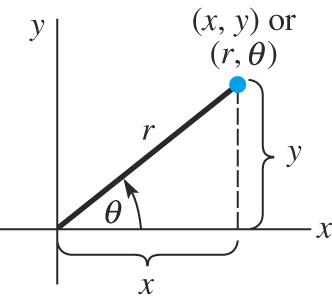
\includegraphics[width=0.5\textwidth]{coordenadas_polares.jpg}		
	\end{figure}
		
	$$r \in [0, \infty),\, \theta \in [0,\, 2\pi]$$
	
	\begin{table}[H]
		\caption{Transformação de coordenadas cartesinas em polares}
		\label{transformacao_coordenadas_cartesianas_polares}
		\centering		
		\begin{tabular}{|lclclcl|}
			$\theta$       & $=$ & $\arctg\left(\dfrac{y}{x}\right)$ & $\Rightarrow$ & $\dfrac{y}{x}$ & $=$ & $\tg(\theta)$     \\
			$\sen(\theta)$ & $=$ & $\dfrac{y}{r}$                    & $\Rightarrow$ & $y$            & $=$ & $r\,\sen(\theta)$ \\
			$\cos(\theta)$ & $=$ & $\dfrac{x}{r}$                    & $\Rightarrow$ & $x$            & $=$ & $r\,\cos(\theta)$
		\end{tabular}		
	\end{table}
	\begin{table}[H]
		\caption{Coordenadas polares a partir das suas correspondentes cartesianas}
		\label{correpondentes_coordenadas_cartesianas_polares}
		\centering		
		\begin{tabular}{|lclclcl|}
			$x^2 + y^2$    & $=$ & $r^2$          & $\Rightarrow$ & $r$      & $=$ & $\sqrt{x^2 + y^2}$                 \\
			$\sen(\theta)$ & $=$ & $\dfrac{y}{r}$ & $\Rightarrow$ & $\theta$ & $=$ & $\arcsen\left(\dfrac{y}{r}\right)$ \\
			$\cos(\theta)$ & $=$ & $\dfrac{x}{r}$ & $\Rightarrow$ & $\theta$ & $=$ & $\arccos\left(\dfrac{x}{r}\right)$
		\end{tabular}		
	\end{table}
	
	\begin{equation*}
		v = \iint_{R(x,y)} f(x,y)\, dxdy = \iint_{R(r,\theta)} f(r\,\cos(\theta),\,r\,\sen(\theta)) r\,drd\theta
	\end{equation*}
	
\section{Relação entre coordenadas cartesinas e esféricas}
	
	\begin{figure}[H]
		\caption{Coordenadas esféricas}
		\label{coordenadas_esfericas}
		\centering
		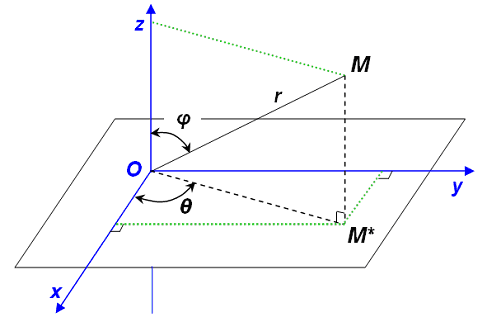
\includegraphics[width=0.5\textwidth]{coordenadas_esfericas.png}		
	\end{figure}
	
	$$r \in [0, \infty),\, \varphi \in [0,\, \pi],\, \theta \in [0,\, 2\pi]$$
	
	\begin{table}[H]
		\caption{Transformação de coordenadas cartesinas em esféricas}
		\label{transformacao_coordenadas_cartesianas_esfericas}
		\centering		
		\begin{tabular}{|lclclcl|}
			$\sen(\varphi)\cos(\theta)$ & $=$ & $\dfrac{x}{r}$ & $\Rightarrow$ & $x$ & $=$ & $r\,\sen(\varphi)\cos(\theta)$ \\
			$\sen(\varphi)\sen(\theta)$ & $=$ & $\dfrac{y}{r}$ & $\Rightarrow$ & $y$ & $=$ & $r\,\sen(\varphi)\sen(\theta)$ \\
			$\cos(\varphi)$             & $=$ & $\dfrac{z}{r}$ & $\Rightarrow$ & $z$ & $=$ & $r\,\cos(\varphi)$
		\end{tabular}		
	\end{table}	
	\begin{table}[H]
		\caption{Coordenadas esféricas a partir das suas correspondentes cartesianas}
		\label{correpondentes_coordenadas_cartesianas_esfericas}
		\centering		
		\begin{tabular}{|lclclcl|}
			$x^2 + y^2 + z^2$ & $=$ & $r^2$                         & $\Rightarrow$ & $r$       & $=$ & $\sqrt{x^2 + y^2 + z^2}$                         \\
			$\tg(\theta)$     & $=$ & $\dfrac{y}{x}$                & $\Rightarrow$ & $\theta$  & $=$ & $\arctg\left(\dfrac{y}{x}\right)$                \\
			$\tg(\varphi)$    & $=$ & $\dfrac{\sqrt{x^2 + y^2}}{z}$ & $\Rightarrow$ & $\varphi$ & $=$ & $\arctg\left(\dfrac{\sqrt{x^2 + y^2}}{z}\right)$
		\end{tabular}		
	\end{table}
	
	\begin{align*}
		v = \iiint_{R(x,y,z)} f(x,y,z)\, dxdydz =\\ \iiint_{R(r,\theta,\varphi)} f(r\,\sen(\varphi)\cos(\theta),\, r\,\sen(\varphi)\sen(\theta),\, r\,\cos(\varphi))\, r^2\sen(\varphi)\, dr d\varphi d\theta
	\end{align*}